
Durant la tempête de Décembre 1999, un arbre s'est brisé en $B$. Son
extrémité $E$ est tombé à 12~m des racines $R$ en faisant un angle
de 30\degres\ avec le tronc (qui est resté perpendiculaire au
sol). Quelle était la hauteur de l'arbre ?

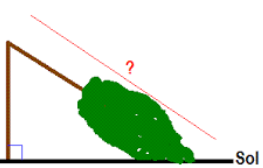
\includegraphics[scale=1]{TR-84.png} 

